\hypertarget{group___linear_interpolate}{}\section{Linear Interpolation}
\label{group___linear_interpolate}\index{Linear Interpolation@{Linear Interpolation}}
Collaboration diagram for Linear Interpolation\+:
\nopagebreak
\begin{figure}[H]
\begin{center}
\leavevmode
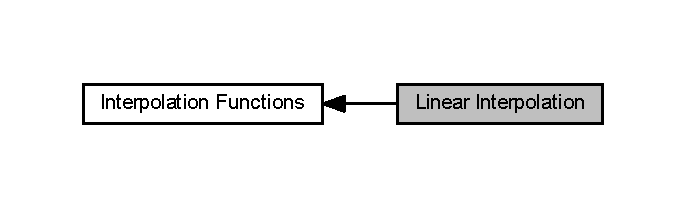
\includegraphics[width=329pt]{group___linear_interpolate}
\end{center}
\end{figure}


\subsection{Detailed Description}
Linear interpolation is a method of curve fitting using linear polynomials. Linear interpolation works by effectively drawing a straight line between two neighboring samples and returning the appropriate point along that line

\begin{DoxyParagraph}{}
 
\end{DoxyParagraph}
\begin{DoxyParagraph}{}
A Linear Interpolate function calculates an output value(y), for the input(x) using linear interpolation of the input values x0, x1( nearest input values) and the output values y0 and y1(nearest output values)
\end{DoxyParagraph}
\begin{DoxyParagraph}{Algorithm\+:}

\begin{DoxyPre}
      y = y0 + (x - x0) * ((y1 - y0)/(x1-x0))
      where x0, x1 are nearest values of input x
            y0, y1 are nearest values to output y
\end{DoxyPre}

\end{DoxyParagraph}
\begin{DoxyParagraph}{}
This set of functions implements Linear interpolation process for Q7, Q15, Q31, and floating-\/point data types. The functions operate on a single sample of data and each call to the function returns a single processed value. {\ttfamily S} points to an instance of the Linear Interpolate function data structure. {\ttfamily x} is the input sample value. The functions returns the output value.
\end{DoxyParagraph}
\begin{DoxyParagraph}{}
if x is outside of the table boundary, Linear interpolation returns first value of the table if x is below input range and returns last value of table if x is above range. 
\end{DoxyParagraph}
